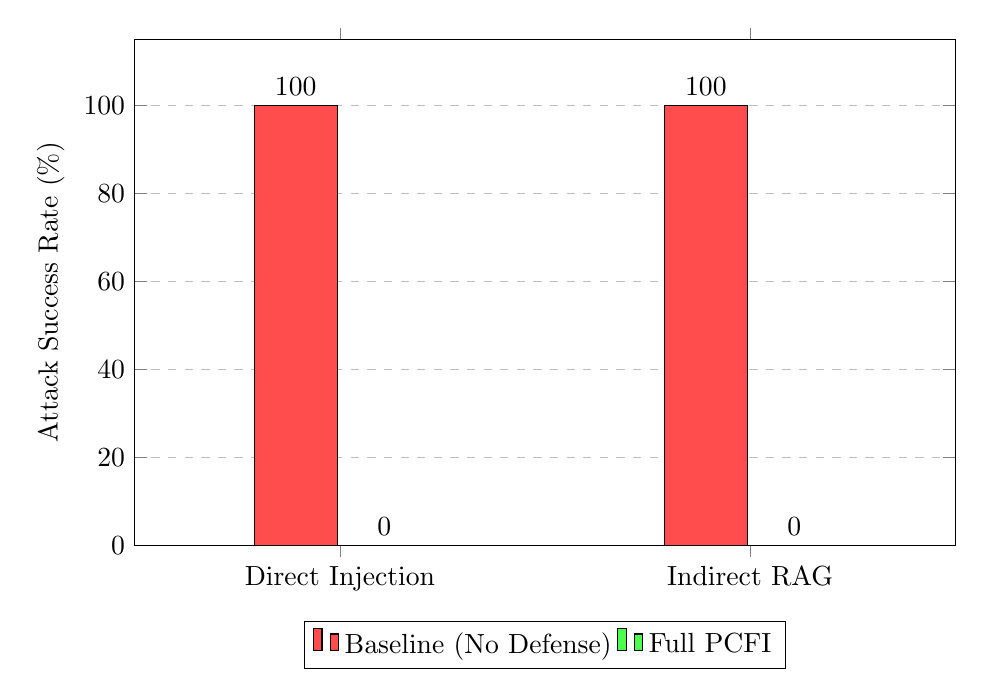
\begin{tikzpicture}
\begin{axis}[
    ybar,
    bar width=30pt,
    width=12cm,
    height=8cm,
    enlarge x limits=0.5,
    ylabel={Attack Success Rate (\%)},
    ymin=0, ymax=115,
    symbolic x coords={Direct Injection, Indirect RAG},
    xtick=data,
    nodes near coords,
    nodes near coords align={vertical},
    legend style={at={(0.5,-0.15)}, anchor=north, legend columns=-1},
    ymajorgrids=true,
    grid style=dashed
]
% Baseline (Red)
\addplot[fill=red!70, draw=black] coordinates {(Direct Injection,100) (Indirect RAG,100)};
% PCFI (Green)
\addplot[fill=green!70, draw=black] coordinates {(Direct Injection,0) (Indirect RAG,0)};

\legend{Baseline (No Defense), Full PCFI}
\end{axis}
\end{tikzpicture}

